\input{configuration}

\title{Lecture 13 --- File Organization }

\author{Jeff Zarnett \\ \small \texttt{jzarnett@uwaterloo.ca}}
\institute{Department of Electrical and Computer Engineering \\
  University of Waterloo}
\date{\today}


\begin{document}

\begin{frame}
  \titlepage

 \end{frame}
 
 

\begin{frame}
\frametitle{File Organization}

A few different file organization options we could choose: 
\begin{multicols}{2}
\begin{enumerate}
	\item \textbf{Heap File}
	\item \textbf{Sorted File}
	\item \textbf{Hashed File}
	\item \textbf{B-Tree File}
\end{enumerate}
\columnbreak
\begin{center}
	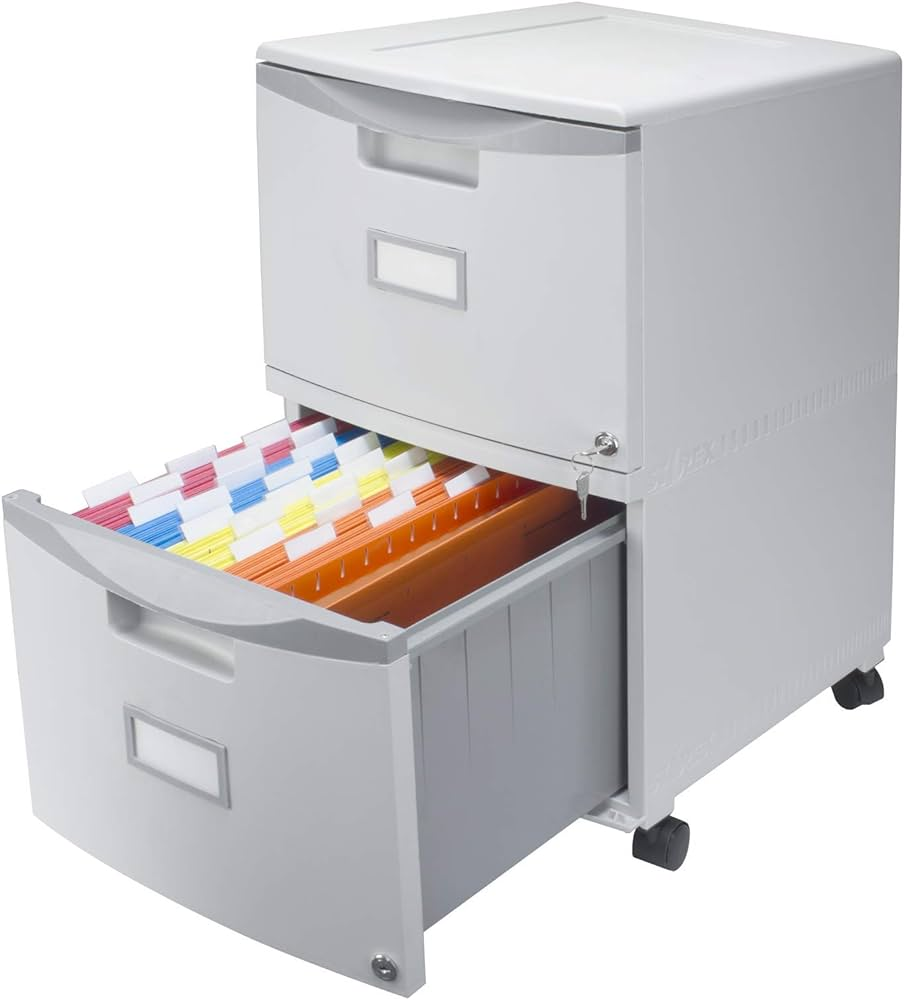
\includegraphics[width=0.3\textwidth]{images/filingcabinet.jpg}
\end{center}
\end{multicols}

\end{frame}



\begin{frame}
\frametitle{File Organization}

Under most circumstances one relation corresponds to one file. 


However, multiple relations can be in the same file if desired. 

To start with, we will just have one relation in a file. 


\end{frame}



\begin{frame}
\frametitle{File Organization}


Remember that these file organizations are not affected by whether records are of fixed or variable length.

The first $k$ records may be stored in the first block, but which records are the first $k$?

\end{frame}


\begin{frame}
\frametitle{Heap File}

The simplest way to order records is: don't order the records! 

\begin{center}
	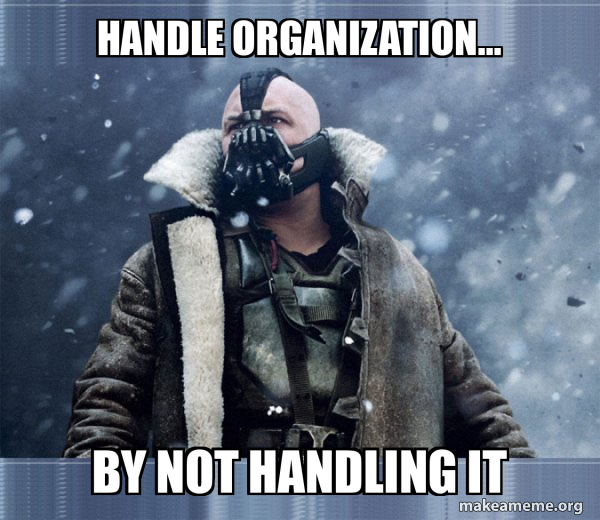
\includegraphics[width=0.4\textwidth]{images/bane.jpg}
\end{center}

The heap file has no inherent organization. 

\end{frame}


\begin{frame}
\frametitle{Heap File}

Records appear in the file in the order in which they are inserted. 

However, there is no guarantee about that, and if that is the behaviour it is an implementation detail and should not be relied upon. 

\end{frame}


\begin{frame}
\frametitle{Heap File}

This strategy makes insertion efficient -- just tack this on to the end of the file, a constant time ($O(1)$) operation. 

If a new block is needed, allocate that new block and write it to disk. 

If not, the last block of the file is read, modified, and written.

\end{frame}


\begin{frame}
\frametitle{Heap File}
However, searching for a record is more difficult, because the file is not ordered.

Thus, we would have to perform a linear search ($O(n)$) over all records. 

\end{frame}


\begin{frame}
\begin{center}
	
\includegraphics[width=0.5\textwidth]{images/detektiv.png}
\end{center}

To find one individual record in the relation it be necessary to examine, on average, half of the entries (assuming that all requests are equally likely).

If the element is not in the file at all then we have to examine all the elements, and it was all for nothing.

\end{frame}



\begin{frame}
\frametitle{Heap File}

To delete a record, we need to first search for the record (linear search), then rewrite the block that it is in. 

Ultimately after enough deletions there will be multiple partially-full blocks, leading to wasted space. 

Thus, compaction of some sort will eventually need to take place which moves the records around to fill in these holes.

\end{frame}


\begin{frame}
\frametitle{Heap File}

An update has all the problems we've discussed before. We must linear search to find the record(s) to the updated. 

It may lead to reorganization of a block or having to move the file to a different block, treating it as if it is an insertion and deletion.  

\end{frame}



\begin{frame}
\frametitle{Heap File General Notes}

Heap organization throws into the light the idea that the file structure has performance implications. 

No matter what we choose, it will mean some operations are faster at the expense of other operations. 

Heap organization means that insertion is fast but reading, updating, and deleting are slower. 

\begin{center}
	
\includegraphics[width=0.5\textwidth]{images/pile.jpg}
\end{center}

Normally we would expect retrieval to be the most common operation, right?


\end{frame}

\begin{frame}
\frametitle{Sorted File}

In a sequential file, we will sort the records based on one particular attribute from start to end.

The field that we sort the file on is called the \alert{ordering field}. 

If it is a  unique key then it is called an \alert{ordering key}.

It does not have to be the primary key.

\end{frame}


\begin{frame}
\frametitle{Sorted File}

A search that is on the ordering field is quite efficient. 

Suppose employees have sequential unique employee ID numbers and that is the ordering key in the database. 

If the goal is to find all employees with an ID less than 385, the data is sequential in all the blocks and that is convenient.

To find an individual record we can use a binary search ($O(\log n)$).

\end{frame}


\begin{frame}
\frametitle{Sorted File}
A simple sequential organization looks like:

\begin{center}
\includegraphics[width=0.7\textwidth]{images/sequential}
\end{center}


\end{frame}



\begin{frame}
\frametitle{Sorted File}

It can be difficult to maintain the physical ordering of the data because every insertion, deletion, update (?) requires a lot of moving records around. 


\begin{center}
\includegraphics[width=0.65\textwidth]{images/sequential-2}
\end{center}

\end{frame}


\begin{frame}
\frametitle{Sorted File}
If the insertion we are doing goes at the end of the file such as in the example an ID of 99001 is inserted, then the file maintains its sequential order. 

If, as in the case shown above, the block is full then we need to place the new record somewhere else. 

For that there is often an \alert{overflow block} where records that do not fit into their normal locations go. 

\end{frame}



\begin{frame}
\frametitle{Sorted File}

Deletion is the mirror image of insertion. 

If we deleted the record at the very end of the file, there is nothing special to maintaining order. 

If the record being deleted is in an overflow block, that makes the order more sequential rather than less. 

\end{frame}



\begin{frame}
\frametitle{Sorted File}

If the record inside a block is being deleted, update the pointers.

The empty space would be noted for the future. 

\end{frame}



\begin{frame}
\frametitle{Sorted File}

If this continues over time, the file loses its sequential ordering as more and more records end up in overflow blocks. 

Eventually the file must be reorganized which sorts the records based on the sequential order again. 

Because this is a potentially expensive operation, it would likely only be done when the system is not busy and when there are enough records out of order.

\end{frame}



\begin{frame}
\frametitle{Hashed File}

A hashed file works very much like the sorted file, except, instead of the sorting key being a number, a hashed value is used instead. 

The hash technique can allow for fast access to records. 

The hash field is often the key. 

\end{frame}

\begin{frame}
\frametitle{Hashed File}

On its own that does not sound any different than the sorted file. 

The ``magic'' in the use of the hash function is that the hashed value tells us the address of the disk block in which the record is stored. 

Instead of having to search to find the record with ID 99901, we could instead compute the hash value and find out that it is in block $x$ and then go there.

\end{frame}



\begin{frame}
\frametitle{Internal Hashing}

We will take a short digression to cover the subject of hashing, actually. 

In Data Structures and Algorithms you learned about \alert{internal hashing}, which we will quickly review, but hashing can be much more.

\begin{center}
	
\includegraphics[width=0.4\textwidth]{images/knowmore.jpg}
\end{center}


\end{frame}


\begin{frame}
\frametitle{Simple Hash Table}

If you implement a hash table simply, there is an array with $M$ ``slots''. 

The hash function turns a particular value into an integer between $0$ and $M-1$. 

The hash function can be as simple as some integer field modulo $M$. 

That algorithm will work but probably does not provide ``nice'' properties to the hash function, or its output. 

\end{frame}


\begin{frame}
\frametitle{Better Hash Table}
It is more likely that you actually want a hash function that has some better properties. 

A \alert{folding} hash function does some arithmetic operations -- add up some numbers, reverse some positions, move blocks around...

Regardless of how the hash function is calculated, we need to deal with the fact that two input values will eventually produce the same output value. 

This is called a \alert{hash collision}.

\end{frame}


\begin{frame}
\frametitle{Many Collisions! HANDLE IT!}

\alert{Open Addressing} -- simply go to the next open space if we must. 

Suppose the hash function computes $n$ but there is already an element stored at that position. 

Then just go to position $n+1$ and put it there (if possible, else go to $n+2$...)

This is simple, but it can lead to clustering, where a bunch of elements are close together.


\end{frame}

\begin{frame}
\frametitle{Chaning}

The next strategy is \alert{chaining}. 

In this case, we have overflow locations. 

If there is a collision, we put the new item in an empty space and put a pointer from one element to the next. 

\end{frame}


\begin{frame}
\frametitle{Multiple Hashing}

The third strategy is a second hash function (\alert{multiple hashing}) that is run if we have a collision to differentiate. 

We could have a third, fourth, etc. function but as one point we will default to open addressing because we will have no other choice.


\end{frame}



\begin{frame}
\frametitle{Hashing Goals}

A goal of hashing is to distribute the records relatively evenly across the address space so that we do not have too many collisions.

We also do not want too much empty space. 

\begin{center}
	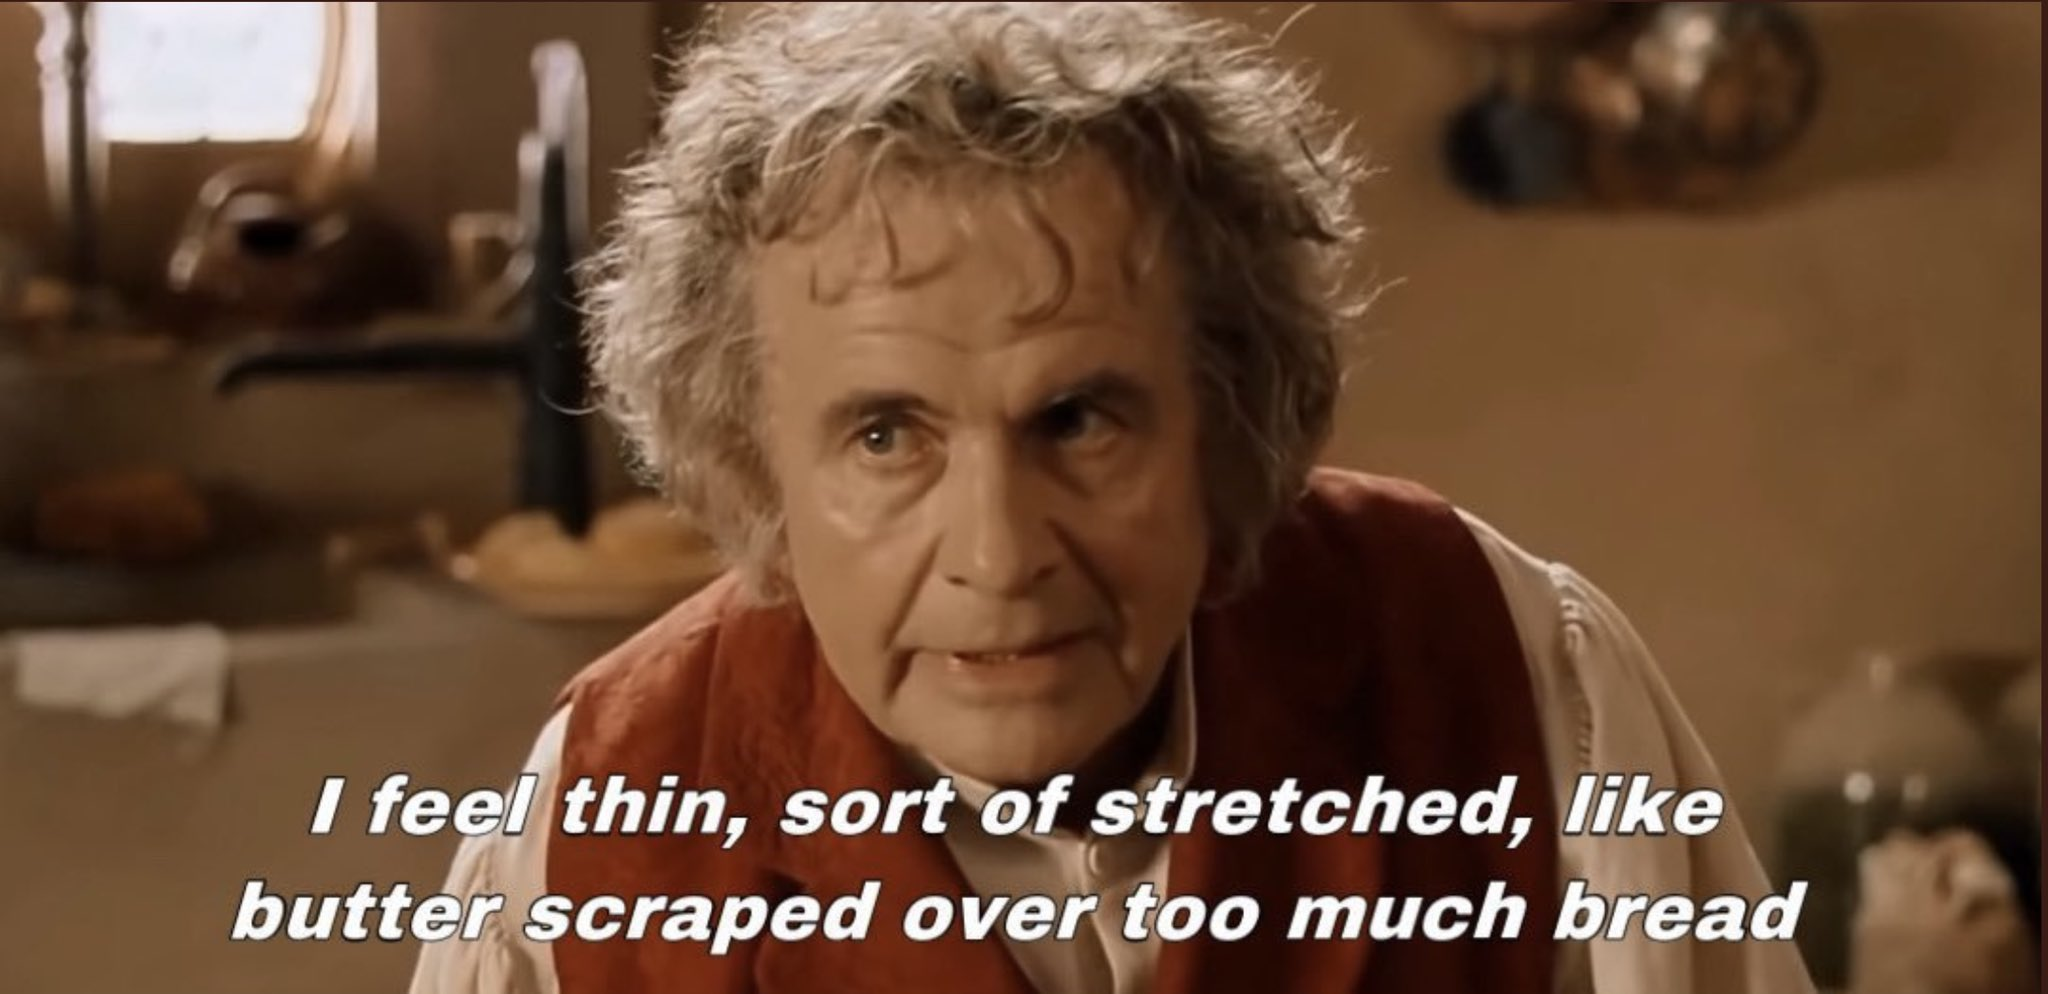
\includegraphics[width=0.4\textwidth]{images/butter.jpg}
\end{center}

Ideal is something like 70-90\% full; and if we need to make the table bigger (or smaller), then we do so.

\end{frame}

\begin{frame}
\frametitle{External Hashing}

With the review of internal hashing aside, we should take a look at external hashing, which is what we need for files on disk. 

Instead of viewing the data storage as an array where we can store one element, instead we have buckets that hold multiple records... 

Then, the hashing function produces a bucket (block) number, and then from there we can get to the actual record by looking in the header for the block.

We will need overflow buckets.

\end{frame}

\begin{frame}
\frametitle{Static Hashing}
Still, all the hashing we have covered so far is \alert{static hashing}, that is to say, we have a fixed number of buckets. 

In a database, files will need to grow as the amount of data in the tables increases (or not be allocated as ridiculously large and mostly empty). 

If most buckets are close to full, we could simply add more buckets and then use a new hashing function to reassign all the items (but this is slow!).

\end{frame}


\begin{frame}
\frametitle{Overflow Buckets}

\begin{center}
	\includegraphics[width=0.9\textwidth]{images/overflow-buckets}
\end{center}

\end{frame}

\begin{frame}
\frametitle{Extendible Hashing}

The first approach is \alert{extendible hashing} -- an access structure is stored in addition to the file. 

The access structure is an array of $2^{d}$ bucket addresses, where $d$ is the global depth of the directory.

\end{frame}

\begin{frame}
\frametitle{Extendible Hashing}

The first $d$ bits of a hash value are the index into the array to determine which element of the array is selected. 

The array element is the bucket in which the corresponding entry is stored. 

Local depth $d'$ specifies the number of bits on which the local bucket contents are based.

\end{frame}

\begin{frame}
\frametitle{Extendible Hashing}

\begin{center}
	\includegraphics[width=0.65\textwidth]{images/extendible-hashing}
\end{center}

\end{frame}


\begin{frame}
\frametitle{Extendible Hashing}

Extendible hashing is great because it allows the file to grow and shrink as is appropriate with the amount of data that is in the file. 

As things get close to full, we just create a new bucket (or several buckets) and the rate of collisions falls again. 

If we have to split a bucket, then a relatively small number of records need to be moved. 


\end{frame}



\begin{frame}
\frametitle{Increasing the Number of Buckets}
If we have to increase the value of $d$ then we have a potentially larger and more painful reorganization, but we probably won't lose any sleep over that. 

Why not? When $d$ is small, the total number of records in the system is not very large so the time to move all of them (worst case) is not very big. 


\end{frame}



\begin{frame}
\frametitle{Increasing the Number of Buckets}

For example, if $d$ is 3, if the table is completely full, there are $2^{3} = 8$ buckets. Not very many. 

If $d$ is large then increasing it is very rare. 

If $d$ is 16 there are $2^{16} = 65~536$ buckets and it takes a long time to fill them up.

\end{frame}




\begin{frame}
\frametitle{B-Trees}

We will assume that everyone is familiar with B-Trees from a data structures and algorithms course (and perhaps a review from an operating systems course...). 

We will actually look into B-Trees in more detail when we talk about the idea of indexing. 

But theoretically we could use B-Trees to store the data in a way that very much resembles how operating systems store files on disk.

\end{frame}



\begin{frame}
\frametitle{Multiple Record Types}

Everything else so far has assumed that each type of record has its own file.

It is possible to keep multiple types of record in the same file, and that could speed up join queries.

In a similar but less extreme variation, we could put tables that we know to be related next to one another on disk.

\end{frame}




\end{document}

